\chapter{Models and Methods}

The models presented in chapter~\ref{relevant-models} seem to work well either in the context of adaptive systems where we are not concerned with timing information or have been tested in controlled environment where the students had no prior knowledge of the presented material. In this chapter, we elaborate the methods we used to further improve the performance by taking into account the timing information of students' answers, i.e. the response times or the age of previous presentations. We are interested primarily in domains where the prior knowledge varies widely between students.

\section{Models Based on Timing Information}
\label{models-timing}

In this section we discuss several models which aim at modeling students' memory with the usage of timing information of answers.

\subsection{The Extended Model}
\label{pfaet}

The extended PFA model summarized in chapter~\ref{pfae} can be further enhanced when we utilize the timing information by locally changing the memory activation in prediction. The difference in seconds between the times of the current question and the last answer is passed to a \textit{time effect function} (we use this term as it was used in a related work~\cite{Pelanek2015}). The time effect function increases or decreases the probability of recall or the memory activation depending on the age of the previous trial. The updated equation with a time effect function is depicted in Equation~\ref{eq-pfa-standard-time-p}.

\begin{equation} \label{eq-pfa-standard-time-p}
  P(m) = \sigma(m + f(t))
\end{equation}

The advantage of this model is that it easy to employ Elo model for estimation of prior knowledge as well as to account for the probability of guessing.

\subsection{The Alternative Model}
\label{pfagt}

Another way of dealing with timing distances between trials is by changing the idea of the model with a decay factor $\xi$ presented in chapter~\ref{pfag}. The model takes into account the order of questions, yet does not consider the ages of student's previous practices. This problem can be resolved by replacing $\xi^{n-k}$ with two time effect functions for correct and incorrect performances.

\begin{equation} \label{eq-pfag-time-s}
  s_{i,j} = \sum_{k=1}^{n-1} y_k \cdot f_{\mathit{succ}}(t_k)
\end{equation}

\begin{equation} \label{eq-pfag-time-f}
  f_{i,j} = \sum_{k=1}^{n-1} |y_k - 1| \cdot f_{\mathit{fail}}(t_k)
\end{equation}

Equations~\ref{eq-pfag-time-s} and~\ref{eq-pfag-time-f} show the incorporation of time effect functions $f_{\mathit{succ}}$ and $f_{\mathit{fail}}$ in the model ($f_{\mathit{succ}}$ for the successful trials and $f_{\mathit{fail}}$ for the failed trials). Each $t_k$ equals the number of seconds that passed between the current and the $k$-th practice. The weight of successes and failures is thus dependent on the ages of the prior practices.

In this model, we also ignore the parameters $\gamma$ and $\delta$ as the weight of each success and failure depends on parameters of the chosen time effect functions. The updated memory activation function $m$ is shown in Equation~\ref{eq-pfag-m}.

\begin{equation} \label{eq-pfag-m}
  m(i,s,f) = \sum_{j \in KCs} \beta_j + s_{i,j} + f_{i,j} 
\end{equation}

As we discussed in the chapter~\ref{pfa}, the problem arises with multiple-choice questions. Another complication is the choice of some good time effect functions that fit the data well.

\subsection{Response Times}
\label{pfart}

The response time of student may indicate student's level of learning. If the student answers quickly, it often implies knowledge at the level of automaticity. We address this phenomenon by increasing the memory activation $m$ after each answered item.

\begin{equation} \label{eq-pfa-extended-rt}
  m \gets \begin{cases}
            m + \gamma \cdot (1 - P(m)) + r_{\mathit{succ}}(t_d), & \text{\textbf{if }} \text{the answer was correct} \\
            m + \delta \cdot P(m) + r_{\mathit{fail}}(t_d), & \text{\textbf{otherwise}}
          \end{cases}
\end{equation}

Equation~\ref{eq-pfa-extended-rt} shows the adjusted update rule with unary functions $r_{\mathit{succ}}$ for correct answer and $r_{\mathit{fail}}$ for incorrect answer---this distinction is necessary since it has been shown that the response time and the probability of correct performance depends on the performance in previous trials~\cite{papouvsekanalysis}. The function argument $t_d$ is the difference between the time the item was presented and the time it was answered (i.e. it is the student's delay).

\section{Quantifying the Quality of Predictions}
\label{metrics}

One way to quantify the quality of model predictions is to use metric functions. A good choice of a metric function is important for accurate evaluation of performance of student models. In our case we are not interested strictly in the correctness of student's answers, the goal is to precisely assess their knowledge. The information of student's knowledge is crucial if we do not want to demotivate the student by too difficult or simple questions. For this purpose a good choice is the Root Mean Squared Error metric (see~Equation~\ref{rmse}) or the less popular Log Likelihood (see~Equation~\ref{ll})~\cite{Pelanek2015a}.

\begin{equation} \label{rmse}
  RMSE = \sqrt{\frac{\sum_{i=1}^n (p_i - y_i)^2}{n}}
\end{equation}

\begin{equation} \label{ll}
  LL = \sum_{i=1}^n y_i \log(p_i) + (1 - y_i) \log(1 - p_i)
\end{equation}

The RMSE metric represents ``error'', its the square root of the sum of all squared differences between predicted values $p_i$ and true values $y_i$ divided by the number of samples in data set. RMSE yields a number between 0 and 1, where 0 represents perfect predictions. LL metric is the logarithm of likelihood, the LL value is a negative number dependent on the size of the data set (the bigger the dataset, the lower LL value is possible). Higher values of LL represent the better predictions.

In domains such as information retrieval or pattern recognition other types of metrics are commonly used which are based on qualitative understanding of errors~\cite{Pelanek2015a} instead of their probabilistic value. An advantage of this type of metrics is that it can be easily used in multi-classification tasks. These metrics, however, depend on a chosen threshold, e.g. in case the threshold is set to $0.5$ the predictions $0.51$ and $0.98$ are classified as positive while predictions $0.49$ and $0.04$ are classified as negative.

\begin{table}[htbp]
  \centering
  \caption{Confusion matrix.}
  \begin{tabular}{ l l c c }
   \toprule[\heavyrulewidth]
   & & \multicolumn{2}{c}{\textbf{Predicted Outcome}} \\
   & & Positive & Negative \\
   \midrule[\heavyrulewidth]
   \multirow{2}{5em}{\textbf{Observed Value}}
   & Positive & True Positive (TP) & False Negative (FN) \\
   & Negative & False Positive (FP) & True Negative (TN) \\
   \bottomrule[\heavyrulewidth]
  \end{tabular}
  \label{table:confusion-matrix}
\end{table}

The Table~\ref{table:confusion-matrix} shows the confusion matrix of binary classifier (i.e. the mislabeling of classes). Once the confusion of classes is calculated, we can derivate for example precision (see~Equation~\ref{precision}) and accuracy (see~Equation~\ref{accuracy}).

\begin{equation} \label{precision}
  \mathit{Precision} = \frac{TP}{TP + FP}
\end{equation}

\begin{equation} \label{accuracy}
  \mathit{Accuracy} = \frac{TP + TN}{TP + FP + TN + FN}
\end{equation}

Even though the precision and accuracy are not very fit in our case as we are more interested in probabilistic understanding of errors, another commonly used metric based on marking predictions as true/false positives/negatives is Area Under the ROC Curve (AUC). In this metric, we measure the performance across all possible thresholds. The result is a number between $0.5$ and $1$, where $1$ represents perfect predictions of the classifier. Note that if all predictions are divided by 2, AUC stays the same, this property is sometimes criticized---hence, it should be used with caution~\cite{Pelanek2015a}.

\section{Parameter Estimation}
\label{parameter-estimation}

The goal of the fitting procedure is to find the optimal parameters that perform well on new samples. In our case this involves maximizing the predictive ability of our student models by discovering the most fitted parameters. In this section we describe the principal algorithms that are suitable for parameter estimation in our thesis.

\subsection{Grid Search}
\label{grid-search}

This technique is used for parameter optimization, it exhaustively generates a grid of all combinations of selected parameter values where each point in the grid is a function value of a chosen objective metric (e.g. RMSE). The fittest combination of parameters is represented by the best score of the metric (e.g. has lowest error). The Figure~\ref{fig-grid-search-rmse-auc} illustrates a result of the grid search algorithm performed on PFA model with two parameters $\gamma$ and $\delta$.

\begin{figure}[htbp]
  \centering
  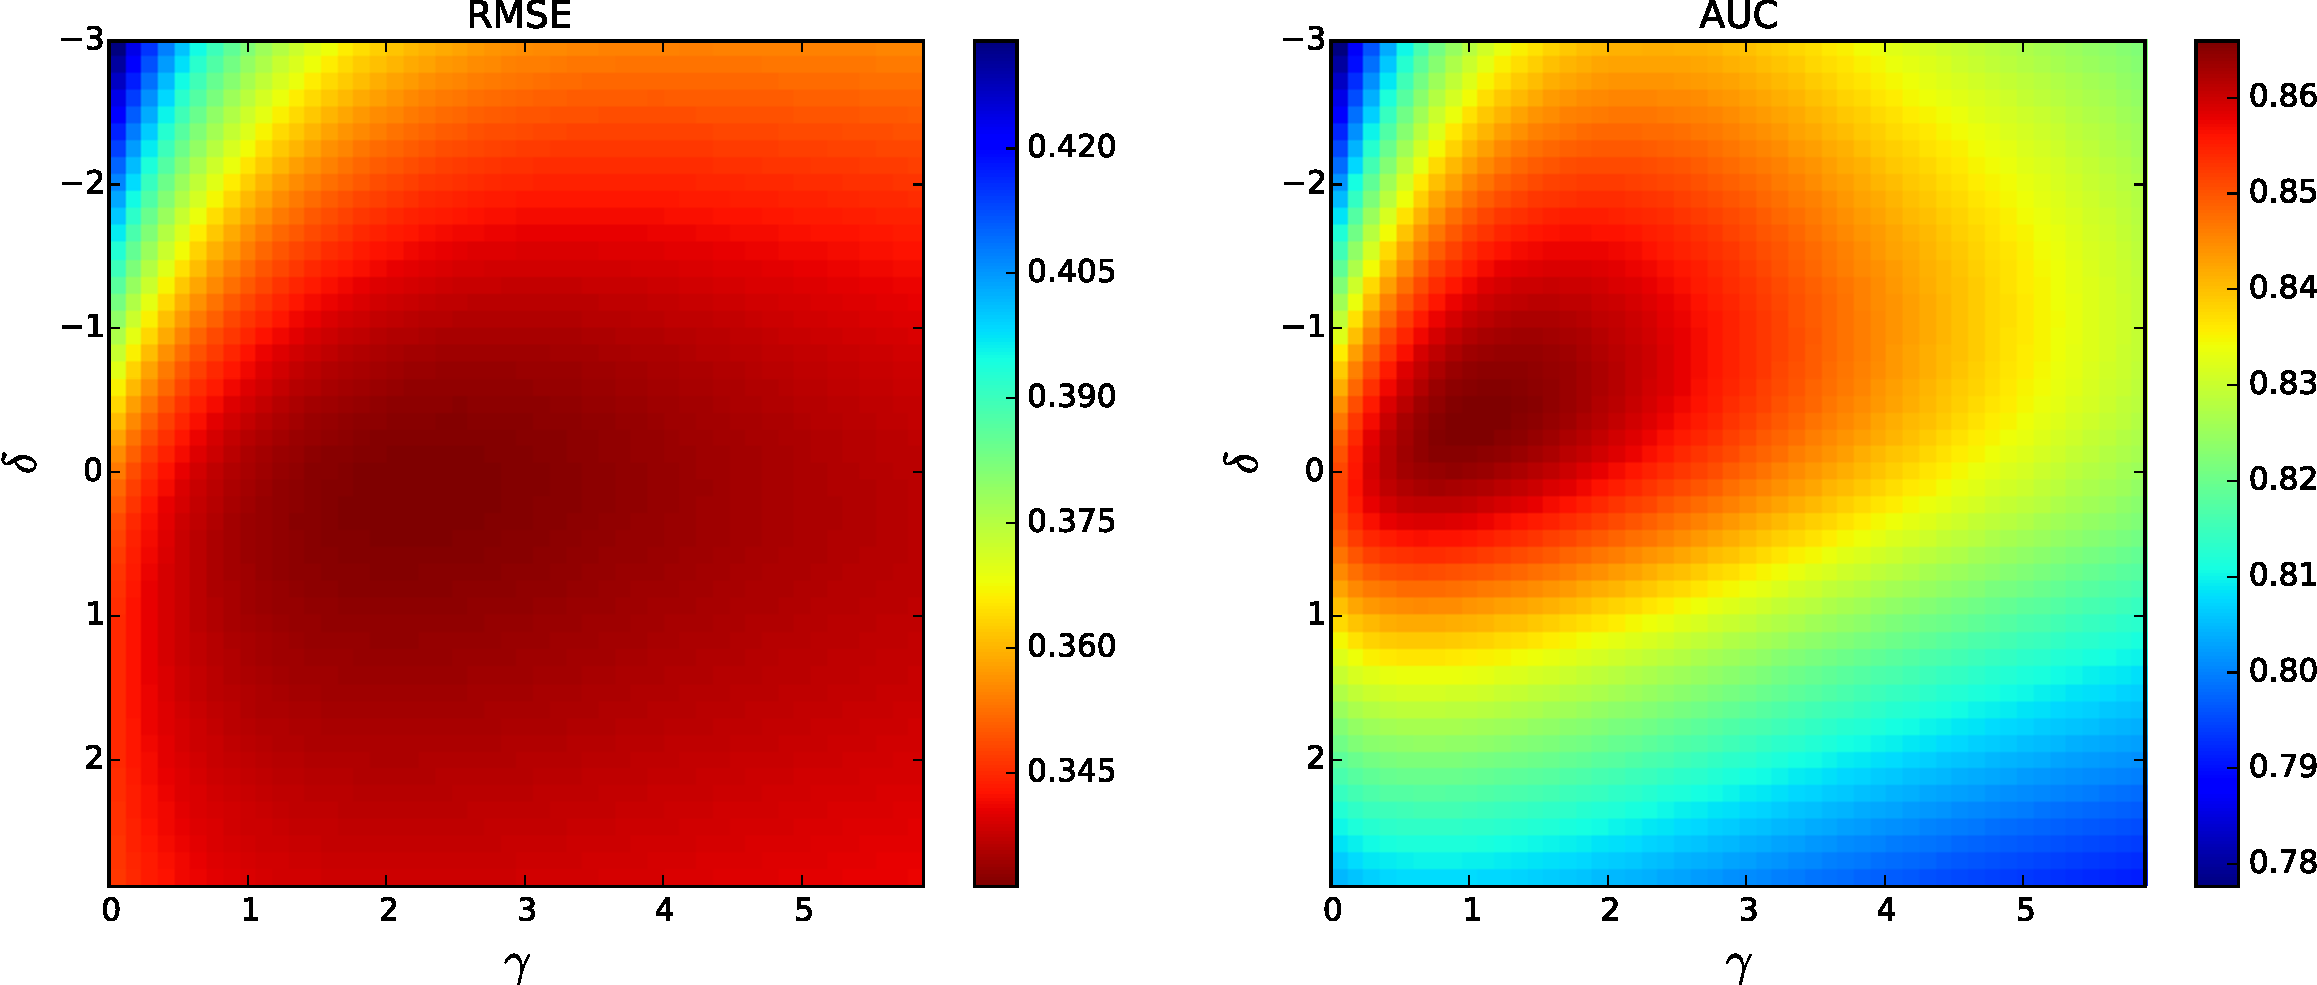
\includegraphics[width=\textwidth]{img/pfa-grid-search-rmse-auc}
  \caption{Result of the grid search performed on the PFA model. The figure shows a grid of model's performance evaluated as RMSE (left) and AUC (right) for each combination of parameters.}
  \label{fig-grid-search-rmse-auc}
\end{figure}

The disadvantage of this optimization method is the high computational complexity especially in cases when the model contains a lot of parameters. Also, there is no simple way to plot or visualize a high-dimensional grid.

\subsection{Hill Climbing}
\label{hill-climbing}

This method starts from a given position in the parameter space and evaluates the score of an objective function (metric function in our case). The model is then trained using the values from the enclosing neighborhood of the parameter space, afterwards the best combination of parameters is selected and the process repeated. This continues until there is no other parameter value in the neighborhood with a better score of the objective function, i.e. in the case of discrete values we found the local minimum, in the case of continuous values we are as close to the local minimum as possible under the preset conditions~\cite{Russell2009}.

\subsection{Gradient Descent}
\label{gradient-descent}

Gradient descent is optimization algorithm very similar to hill climbing, the difference is that gradient descent has indication which way to ``climb''. The goal of gradient descent is to find the best parameters for a function called hypothesis~\cite{Klusasek2014}, this is done by finding the lowest value of the cost function $J(\mathbf{w})$ (or the objective function). The cost function represents the error of a chosen hypothesis $h_{\mathbf{w}}(\mathbf{x}_i) = \mathbf{w}^T \mathbf{x}_i = \sum^n_{j=0} w_j x_{i,j}$, where $w_j$ is the value of the $j$-th parameter and $x_{i,j}$ the $i$-th value of the $j$-th feature (e.g. the skill of the student $i$).

\begin{equation} \label{cost-function}
  J(\mathbf{w}) = \frac{1}{2m} \sum^m_{i=1} (h_{\mathbf{w}}(\mathbf{x}_i) - y_i)^2
\end{equation}

Formal definition of the cost function is depicted in Equation~\ref{cost-function}, it is the sum of all squared errors of hypotheses $h_{\mathbf{w}}$ over all examples from data set of size $m$ divided by $2m$. Our goal is to minimize the value of $J(\mathbf{w})$ which can be done efficiently by the estimation of the gradient using the following update rule:

\begin{equation} \label{cost-function-update}
  w_j \gets w_j - \alpha \frac{\partial}{\partial w_j} J(\mathbf{w})~~\text{for all } j
\end{equation}

The partial derivatives help indicate the surface of the cost function, it gives us the information which direction to take in order to reach the closest local minimum. The value of $\alpha$ is the size of one step also called the learning rate, if the value is too big the algorithm might not be able to ever reach a local minimum, on the other hand if the value is too small, it is less efficient and the computation takes longer. Notice that the main difference between gradient descent and hill climbing is that the latter does not have any indication of which direction to take next and how big one step in that direction should be~\cite{Russell2009}.

\begin{figure}[htbp]
  \centering
  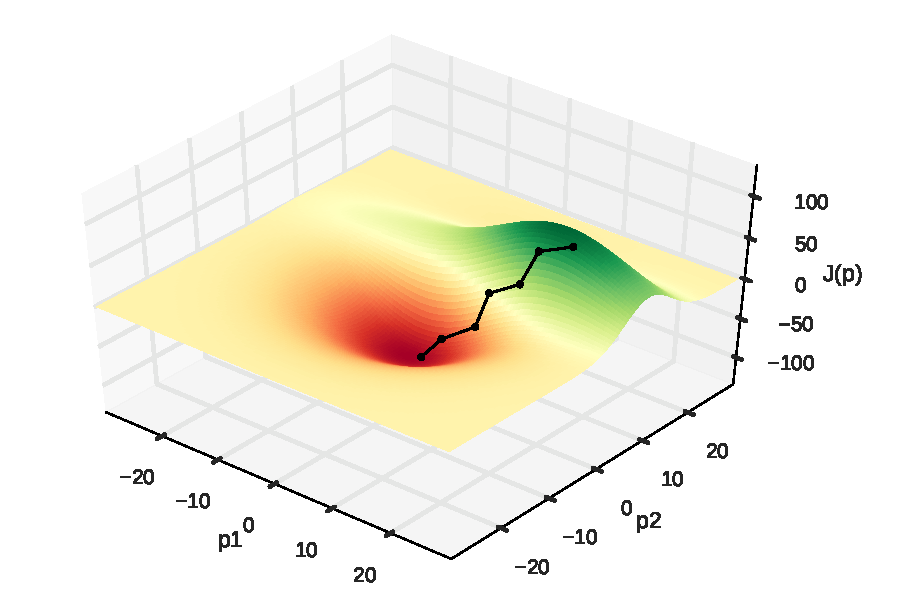
\includegraphics[width=\textwidth]{img/gradient-descent}
  \caption{3D visualization showing first 7 iterations of gradient descent applied to an example with two parameters.}
  \label{fig-gradient-descent}
\end{figure}

\subsection{Approximating the Gradient}
\label{approx-gradient}

In this chapter we discuss possible approximations of the gradient descent to optimize parameters of the PFA model and its variations. The most obvious and easiest way to implement approximate gradient could average the difference between correctness of student's answer $y_i$ and model's predicted probability $p_i$ that the item $i$ is answered correctly. The batch update rule would be defined as follows:

\begin{equation} \label{online-learning-batch-rule}
 w_j \gets w_j - \alpha~\frac{1}{n}\sum_{i=0}^n (p_i - y_i)~~\text{for all } j
\end{equation}

This method has several problems. First, it is easy to demonstrate that it does not work well even in cases where the number of parameters is very low. The parameters get stuck in local minimum can be observed in Figure~\ref{pfa-dummy-gd-step-vs-grid}, e.g. different values of the step size $\alpha$ lead to different values of the parameters $\gamma$ and $\delta$. Another disadvantage of this technique is that the whole process of parameter optimization has to run periodically, which is of course not very desirable in online learning.

\begin{figure}[htbp]
  \centering
  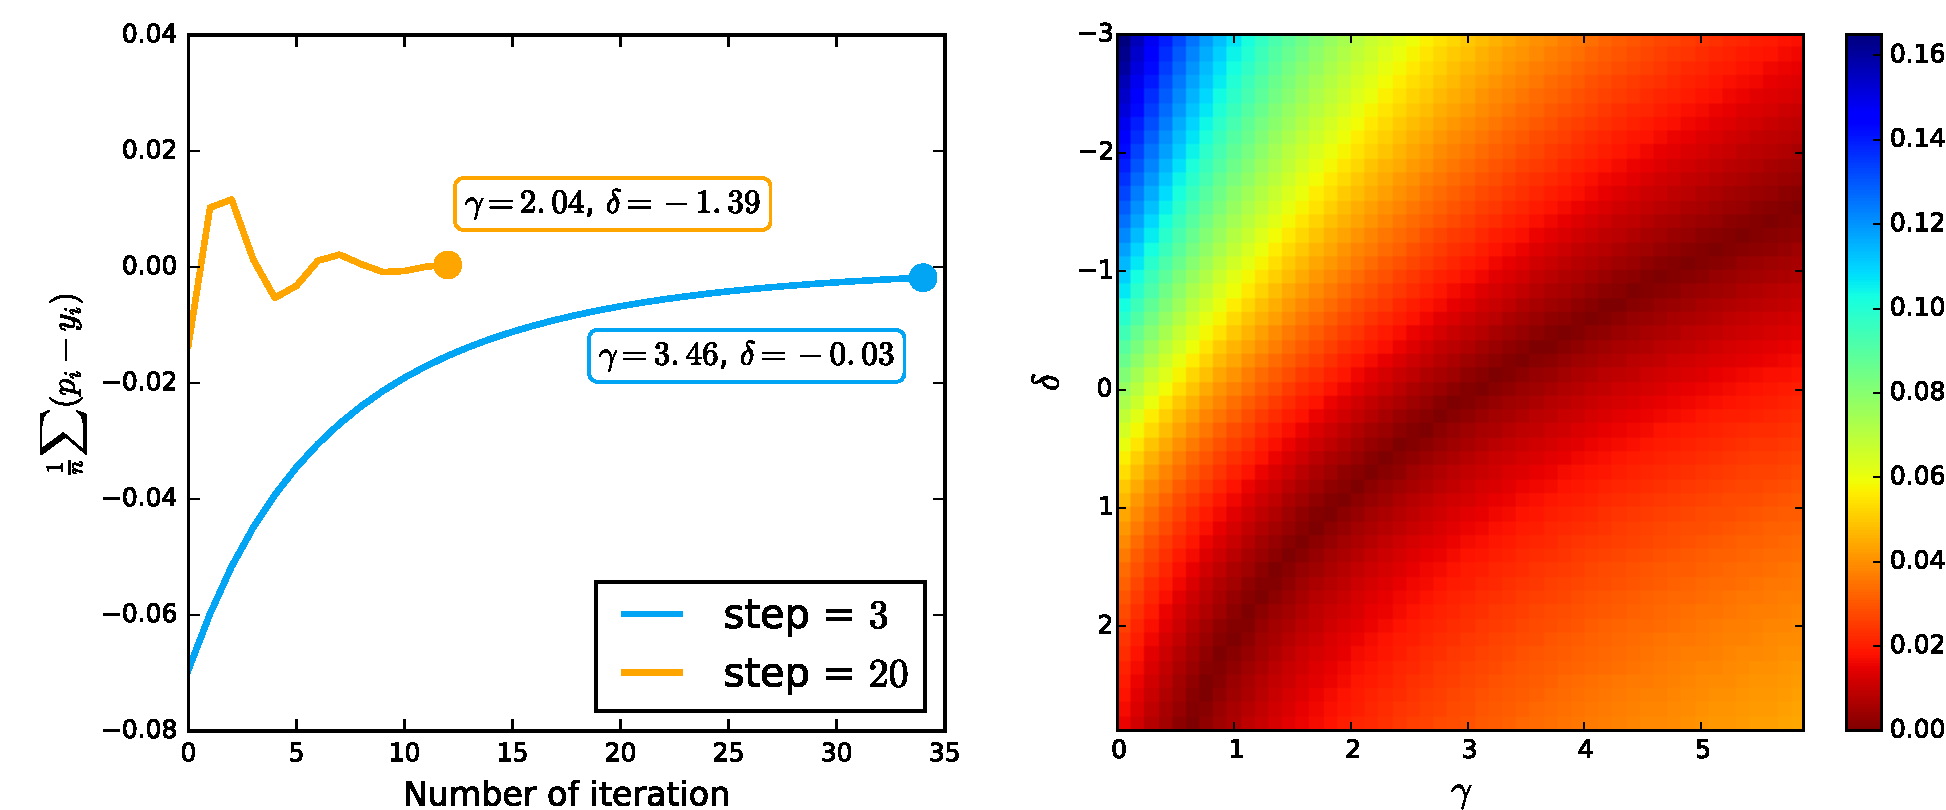
\includegraphics[width=\textwidth]{img/pfa-dummy-gd-step-vs-grid}
  \caption{Demonstration of the flaws of the naive gradient descent. Figure on the left hand size shows two runs with different values of $\alpha$. Figure on the right hand size shows absolute value of $\frac{1}{n}\sum_{i=0}^n (p_i - y_i)$ for a grid of parameters.}
  \label{pfa-dummy-gd-step-vs-grid}
\end{figure}

Radek Pelánek in his work~\cite{Pelanek2015} figured out a bit more complicated way of parameter estimation which combines some aspects of gradient descent and is suitable in online learning. The update of parameters happens after arrival of every new data point (i.e. student's answer). This method is very practical particularly in our case where we need to find the most optimal and best calibrated time effect function.

The Algorithm~\ref{alg-gradient-descent} shows an update of parameters in PFA model with two parameters $\gamma$ and $\delta$. The update is performed whenever a question is answered by a student. To understand the idea of this method, we can examine four possible situations:

\begin{itemize}
  \item $A$ was correct and $P(m) > 0.5$ -- memory activation $m$ is low and should be increased (e.g. by increasing $\gamma$ or $\delta$)
  \item $A$ was correct and $P(m) \leq 0.5$ -- memory activation $m$ is very low and should be greatly increased (e.g. by increasing $\gamma$ or $\delta$)
  \item $A$ was incorrect and $P(m) \leq 0.5$ -- memory activation $m$ is high and should be decreased (e.g. by decreasing $\gamma$ or $\delta$)
  \item $A$ was incorrect and $P(m) > 0.5$ -- memory activation $m$ is very high and should be greatly decreased (e.g. by decreasing $\gamma$ or $\delta$)
\end{itemize}

The process of updating the parameters is repeated for all answers, i.e. it tries to approximate the optimal combination of parameter values by minimizing discrepancy in the above situations.

\begin{algorithm}
  \caption{The algorithm demonstrates update of parameters after one trial of the item $I$. The function expects the practiced item $I$ and current values of global parameters $\gamma$ and $\delta$. Output is a tuple of updated $\gamma$ and $\delta$. Note that $w_{\gamma}$ and $w_{\delta}$ help indicate how much to change activation $m$ of the item $I$ given the previous values of $P(m)$ and student's answers.}
  \label{alg-gradient-descent}
  \begin{algorithmic}[1]
    \Function{UpdateParameters}{$I, \gamma, \delta$}
      \State $m \gets$ \Call{Activation}{$I$} \Comment{Returns memory activation of the item $I$.}
      \State $A \gets$ \Call{LastAnswer}{$I$} \Comment{Returns the last practice of the item $I$.}
      \If{\Call{IsCorrect}{$A$}} \Comment{Checks correctness of the last answer.}
        \State $s \gets 1 - P(m)$
      \Else
        \State $s \gets 0 - P(m)$
      \EndIf
      \State $w_{\gamma}, w_{\delta} \gets$ \Call{GetWeights}{$I$} \Comment{Returns $w_{\gamma}, w_{\delta}$ local for the item $I$.}
      \State $\gamma \gets \gamma + \alpha \cdot s \cdot w_{\gamma}$ \Comment{The parameter $\alpha$ is the learning rate.}
      \State $\delta \gets \delta + \alpha \cdot s \cdot w_{\delta}$
      \If{\Call{IsCorrect}{$A$}}
        \State $w_{\gamma} \gets w_{\gamma} + s$
      \Else
        \State $w_{\delta} \gets w_{\delta} + s$
      \EndIf
      \State \Call{SetWeights}{$I, w_{\gamma}, w_{\delta}$} \Comment{Updates $w_{\gamma}, w_{\delta}$ locally for the item $I$.}
      \State \Return $\gamma, \delta$
    \EndFunction
  \end{algorithmic}
\end{algorithm}

The process of change of parameters in PFA model using this method is visualized in Figure~\ref{gradient-descent-iterations}. We can also notice that with each iteration of the algorithm, the parameters are updated while error in predictions as measured by RMSE generally decreases.

\begin{figure}[htbp]
  \centering
  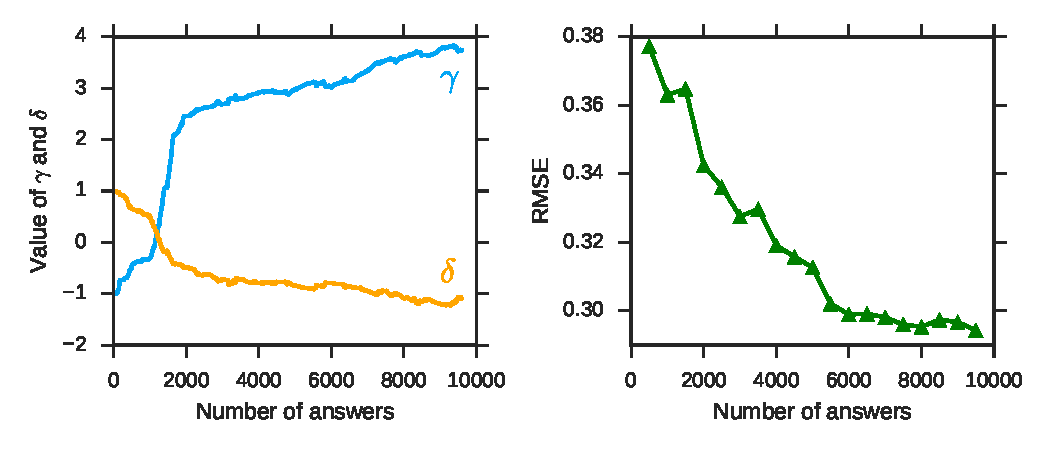
\includegraphics[width=\textwidth]{img/gradient-descent-iterations}
  \caption{Iterations of the algorithm based on gradient descent for parameter estimation in PFA model. The figure on left shows the progress of $\gamma$ and $\delta$ with each new answer. The figure on right indicates the improvement of predictive ability of the model by measuring RMSE each time 500 places are answered by students.}
  \label{gradient-descent-iterations}
\end{figure}

\section{Time Effect Functions}
\label{time-effect-functions}

The goal of a time effect function is to locally increase student's memory activation $m$ of the practiced item while taking into account the time a previous trial of the item was performed. A time effect function thus increases memory activation based on the age of the last answer. For our purpose, we have chosen the following functions with parameter $t$ representing the time of the last presentation and two parameters $a$ and $c$:

\begin{itemize}
  \item $f_{\mathit{log}}(t) = a - c \cdot \log(t)$
  \item $f_{\mathit{exp}}(t) = a \cdot e^{-c \sqrt{t}}$
  \item $f_{\mathit{pow}}(t) = a / t^c$
\end{itemize}

These functions were chosen as simple candidates with only a few parameters, other candidates we experimented with were just similar variations and didn't improve the performance of our models in any significant way. The shape of each of these time effect functions with logarithmically scaled $x$-axis is depicted on Figure~\ref{fig-time-effect-functions}.

\begin{figure}[htbp]
  \centering
  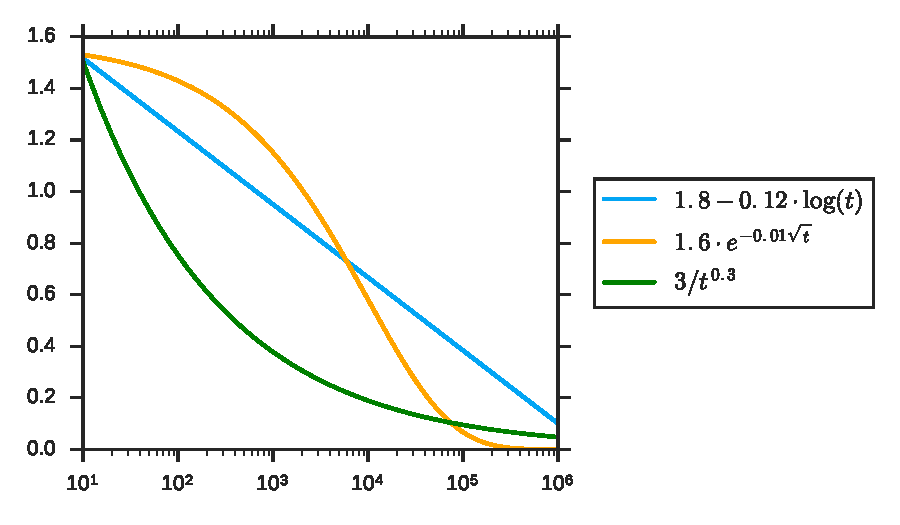
\includegraphics[width=\textwidth]{img/time-effect-functions}
  \caption{Candidates of time effect functions we inspected and evaluated in our analysis. Note that the $x$-axis is log scaled.}
  \label{fig-time-effect-functions}
\end{figure}

\subsection{The Staircase Function}
\label{staircase-function}

If we want to approximate the exact shape of a time effect function, we can define a staircase function with fixed intervals $\mathbf{i}$. In each interval $(i_j, i_{j+1}]$, we preserve a learned value $a_j$ which represents an increase in memory activation. The formal definition of the staircase function $f_{\mathit{staircase}}$ is formalized in Equation~\ref{eq-staircase}.

\begin{equation} \label{eq-staircase}
  f_{\mathit{staircase}}(t) = \begin{cases}
            a_1, & \text{if } i_0 < t \leq i_1 \\
            a_2, & \text{if } i_1 < t \leq i_2 \\
                 & \hspace{1em} \dots \\
            a_n, & \text{if } i_{n-1} < t \leq i_n
         \end{cases}
\end{equation}

Applying simple linear algebra, we can further modify the staircase function so that the memory activation between two points is a linear function, this makes a better approximation of the learned values. The definition of the adjusted function is described in Equations~\ref{eq-staircase-iota-prime-definiton} and~\ref{eq-staircase-linear}, where $T$ is a set of ages of all answers in seconds.

\begin{equation} \label{eq-staircase-iota-prime-definiton}
\begin{split}
  \hat{i}_0 &= i_0 \\
  \hat{i}_j &= \mathit{mean}\{t \in T~|~i_{j-1} < t \leq i_j\}
\end{split}
\end{equation}

\begin{equation} \label{eq-staircase-linear}
  f_{\mathit{staircase}}(t) = \begin{cases}
            a_1, & \text{if } \hat{i}_0 < t \leq \hat{i}_1 \\
            (t - \hat{i}_1) \frac{a_2 - a_1}{\hat{i}_2 - \hat{i}_1} + a_1, & \text{if } \hat{i}_1 < t \leq \hat{i}_2 \\
            \hspace{9em} \dots \\
            (t - \hat{i}_{n-1}) \frac{a_n - a_{n-1}}{\hat{i}_n - \hat{i}_{n-1}} + a_{n-1}, & \text{if } \hat{i}_{n-1} < t \leq \hat{i}_n     
         \end{cases}
\end{equation}

Note that $\hat{i}_0$ is in our case always equal to $0$ and $\hat{i}_n$ to infinity (in which case the memory activation in the interval is equal to $a_n$).
